\chapter{Data reduction} \label{ch:data_reduction}

\textit{The work presented in this chapter is part of a larger study:}

\textbf{MELCHIORS: The Mercator Library of High Resolution Stellar Spectroscopy}

P. Royer, \textbf{K. Dsilva}, T. Merle, S. Sekaran, H. Van Winckel, Y. Fr\'emat, M. Laverick, M. Abdul Masih, B. Acke, M.L. Alonso, S. Bandhu Mahoto, P. Beck, N. Behara, S. Bloemen, B. Buysschaert, N. Cox, J. Debosscher, P. De Cat, P. Degroote, R. De Nutte, K. De Smedt, B. de Vries, L. Dumortier, A. Escorza Santos, K. Exter, S. Goriely, N. Gorlova, H. Hensberghe, M. Hillen, W. Homan, M. Hrudkova, D. Kamath, R. Karjalainen, P. Lampens, R. Lombaert, P. Marcos Arenal, J. Menu, F. Merges, E. Moraweji, P. Nemeth, P. Neyskens, R. Ostensen, P. Papics, J. Perez, S. Prins, A. Samadi, H. Sana, A. Sans Fuentes, S. Scaringi, V. Schmid, L. Siess, C. Siopis, K. Smolders, S. Sodor, A. Thoul, A. Tkachenko, S. Triana, B. Vandenbussche, M. Van der Swaelmen, M. Van de Sande, G. Van De Steene, S. Van Eck, P. van Hoof, A.J. Van Marle, T. Van Reeth, L. Vermeylen, D. Volpi, J. Vos and C. Waelkens

Soon to be submitted to Astronomy \& Astrophysics

\textbf{Author contributions:} The campaign and the assembly of the library was led by P. Royer. K. Dsilva developed the telluric correction and implemented the instrumental response correction for the HERMES pipeline, with guidance and regular discussions with H. Sana, P. Royer and H. Van Winckel. S. Sekaran and T. Merle obtained models for the spectrophotometric standards. All other co-authors conducted a significant amount of observations for the spectral library with the HERMES spectrograph. 

\section{Introduction}

The spectroscopic data used in this thesis was obtained with the High Efficiency, high-Resolution Mercator Echelle Spectrograph \citep[HERMES,][]{raskin_hermes_2011}. As WR stars do not have any continuum, normalising their spectra is challenging, and is usually possible with stellar model atmospheres. However, the pipeline of HERMES does not provide flux-calibrated spectra and hence the shape of the delivered scientific spectra are heavily impacted by that of the response curve of the instrument. In order to circumvent this, we developed a methodology to correct for the instrumental response. The resulting spectrum is a scaled version of the spectral energy distribution, with a contribution from interstellar reddening. In this chapter, the data reduction process is explained in detail. 

\subsection{Instrumental response function}
At the entrance of the telescope, any stellar spectrum S can be decomposed into a number of factors: 
\begin{equation}
    S = C .\ N .\ A^e .\ A^m
\end{equation}
where $A^e$ is the atmospheric extinction, $A^m$ the molecular absorption by the Earth's atmosphere, and $S^0 = C . N$ is the stellar spectrum. Finally $C$ represents the stellar continuum, i.e. the ratio between $S^0$ and the normalised spectrum $N$. The spectrum $S$ contains the effect of the interstellar absorption, which is not corrected for and is consequently included in $C$. In the present work, we produce three types of data products: the response-corrected spectra before and after correction for the telluric bands: $S^{atm}_{OBJ} \triangleq C\,.\,N\,.\,A^m$ and $S^0_{OBJ} \triangleq C\,.\,N$ respectively, and the normalised spectra $N$.

To achieve this, we considered three types of measurements: observations of scientific targets ($f_{obj}$), observations of spectrophotometric calibrators ($f_{cal}$), and flat field exposures ($ff_{raw}$). After the subtraction of the electronic offset, these can be expressed as:
    \begin{align}
    \label{eq:obj}
    f_{obj} &= S_{OBJ} .\, \Re'\\
    \label{eq:cal}
    f_{cal} &= S_{CAL} .\, \Re'\\
    \label{eq:ff}
    ff_{raw} &= FF_{SED} .\, \Re'
    \end{align}
where $FF_{SED}$ expresses the spectral energy distribution (SED) of the flat-field signal, imposed by the spectrum of the lamps and filters used for these measurements. The instrumental response is defined by $\Re' = \Re .\, B .\, P$, in which $B$ represents the blaze function driving the response inside every order of the echelle spectrometer, $P$ is the pixel response non uniformity, and $\Re$ (hereafter called the response) captures the remaining instrumental effects (quantum efficiency of the detector, transmission and reflection of the optical elements, etc.). 

The response $\Re$ is wavelength and time dependent. The wavelength dependence describes the relative spectral response function and the time dependence takes into account possible variations of the environmental conditions (temperature, atmospheric pressure and humidity), instrument aging and in our case residuals with respect to the average atmospheric extinction (see below). Formally, the response encapsulates the flux calibration coefficient, which is disregarded here as HERMES spectra are not calibrated in flux. 

The flat-field exposures are usually acquired at the beginning and at the end of the night. The spectrophotometric calibrators are celestial targets whose absolute spectra are known from accurate modelling. One such object was observed every night whenever possible. We used them to determine and correct for the instrumental response (Sect.~\ref{sec:responsecorr}).

\section{HERMES Pipeline}
The raw 2-D echelle spectra are first processed with the standard HERMES pipeline, which includes bias correction, background subtraction, flat-field correction, cosmic-ray clipping and, order merging \citep{raskin_hermes_2011}. The flat-field correction is a mandatory step to remove the pixel response non
uniformity, but also, prior to order merging, to remove the effect of the blaze function in every order. Dividing by the flat-field is nevertheless artificially imposing the shape of $1 / FF_{SED}$ onto every spectrum thus corrected. The output of the pipeline hence consists in 1-D spectra still affected by the effects of the Earth's atmosphere and the newly introduced shape of the flat-field. 

% \begin{comment}
% Our 1-D spectra now indeed correspond to:
%     \begin{align}
%     \label{eq:divffobj}
%     %f_{obj}^{FF} &= \frac{f_{obj}}{ff} &= \frac{S_{OBJ} .\, \Re}{ff}\\
%     %f_{cal}^{FF} &= \frac{f_{cal}}{ff} &= \frac{S_{CAL} .\, \Re}{ff}
%     f_{obj}^{FF} &= \frac{S_{OBJ} .\, \Re}{ff}\\
%     \label{eq:divffcal}
%     f_{cal}^{FF} &= \frac{S_{CAL} .\, \Re}{ff}
%     \end{align}

% Equations~\ref{eq:divffobj} and~\ref{eq:divffcal}.
% \end{comment}
\begin{table}[ht]
\centering
\caption{Wavelength ranges and the respective molecules included in the fitting process with Molecfit.}
\begin{tabular}{ccl}
\hline \hline
Wavelength start (\AA) & Wavelength end (\AA) & Molecule \\
\hline
6274 & 6324 & O$_2$     \\
6850 & 7074 & O$_2$ (B band)     \\
7227 & 7269 & H$_2$O    \\
7589 & 7714 & O$_2$ (A band)    \\
8101 & 8344 & H$_2$O    \\
8940 & 8971 & H$_2$O    \\
\hline
\end{tabular}
\label{tab:molecfitranges}
\end{table}

\subsection{Atmospheric extinction and telluric correction}
\label{sec:atm_corr}
To correct for the atmospheric extinction $A^e$, a wavelength and airmass-dependent atmospheric correction is applied following tabulated values for the Roque de Los Muchachos Observatory on the island of La Palma\footnote{https://www.ing.iac.es/Astronomy/observing/manuals/html\_manuals/general/obs\_guide/node293.html}. This correction is an average: it slightly varies in cases where the observations were carried out under conditions of thin clouds and also strongly depends on the nature and quantity of dust along the atmospheric line-of-sight. However, the spectra obtained for the RV monitoring campaign were obtained on clear nights, and so this does not seem to be a problem.

To correct for the telluric line absorption $A^m$, we use the publicly available tool Molecfit \citep{smette_molecfit_2015,kausch_molecfit_2015}. By combining essential input from the Mercator meteo-station with a molecular line database and a radiative transfer code, Molecfit models the instrument line spread function and atmospheric content at the time of the observation. The wavelength ranges and molecules included in the fitting procedure are listed in Table\,\ref{tab:molecfitranges}. For every region included in the fit, the continuum is estimated locally using a first order polynomial. Molecfit also corrects for any minor wavelength shifts by fitting the wavelength solution with a second order Chebyshev polynomial. 

After correction, the spectra show residuals of $\sim\!\!5\%$ (Fig. \ref{fig:tell_corr_7227}) of the continuum in the telluric bands, with the exception of the saturated lines. While fitting saturated lines, the division of two numbers close to zero often results in large residuals (the oxygen band around $7600\,$\r{A}, is often impacted this way). In the region after $8950\,$\r{A} we observe residuals due to a small imperfection of the wavelength calibration solution at the red edge of the spectra (Fig. \ref{fig:tell_corr_8940}).

\begin{figure}
    \centering
    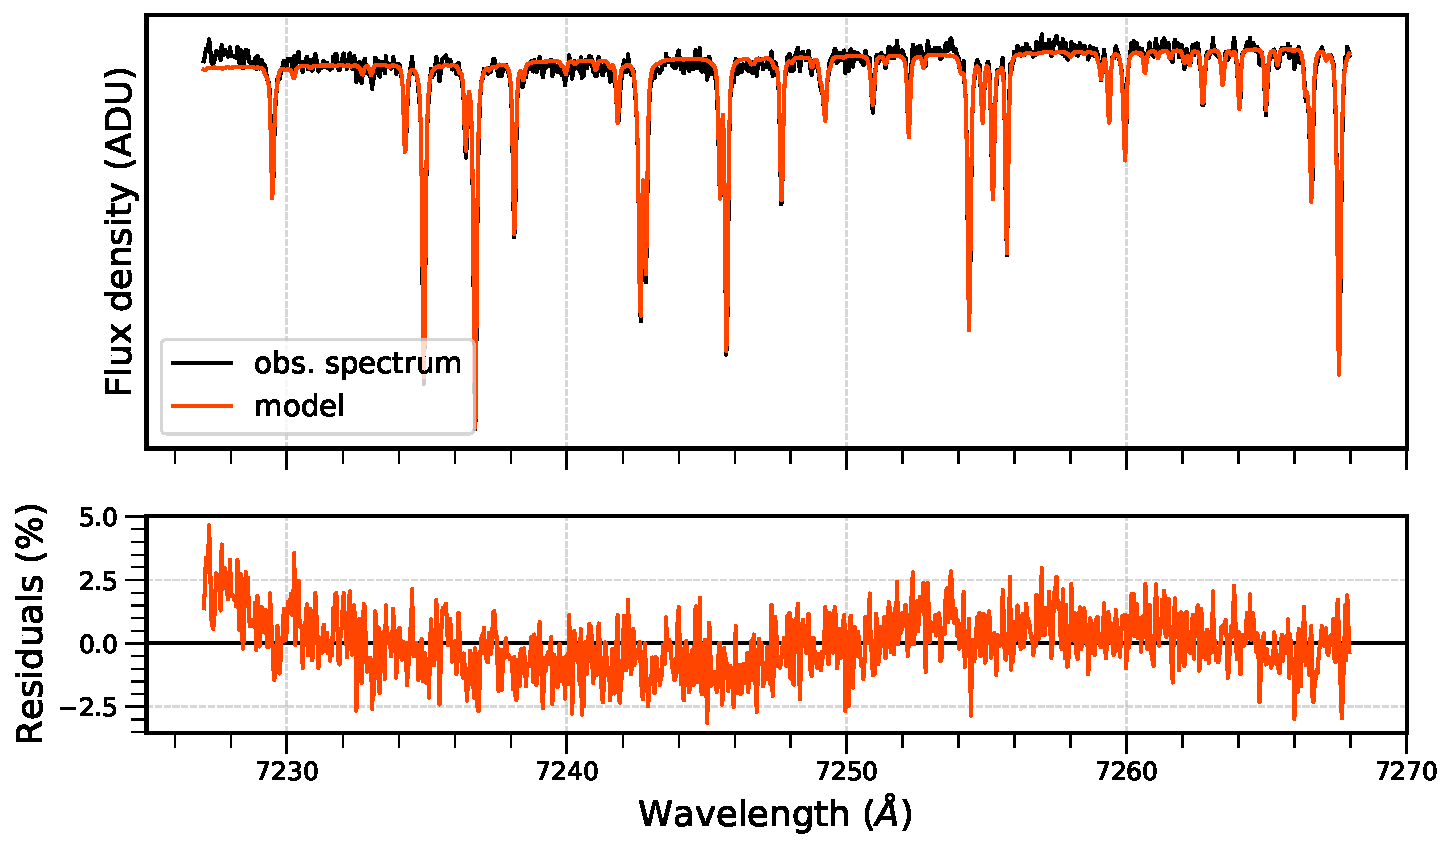
\includegraphics[width=\hsize]{chapters/data_reduction/image/tell_corr_7227_7268.pdf}
    \caption{Telluric correction of WR 136 (WN6b(h)) in the region 7227\,\r{A} to 7269\,\r{A}, showing residuals less than 5\%.}
    \label{fig:tell_corr_7227}
\end{figure}

\begin{figure}
    \centering
    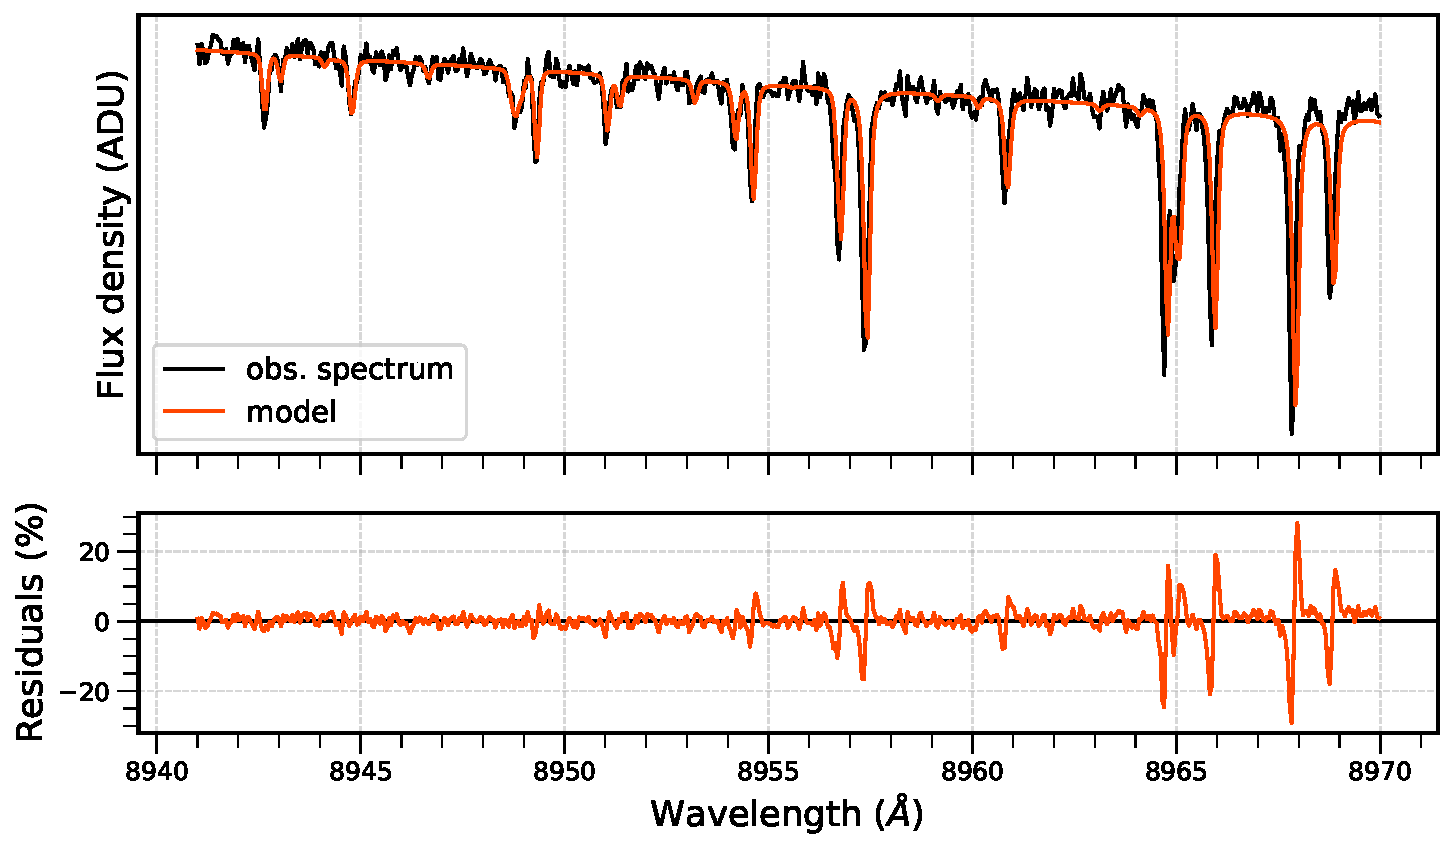
\includegraphics[width=\hsize]{chapters/data_reduction/image/tell_corr_8940_8970.pdf}
    \caption{Telluric correction of WR 136 (WN6b(h)) in the region 8940\,\r{A} to 8970\,\r{A}. The uncertain wavelength calibration causes residuals of the order  20\%.}
    \label{fig:tell_corr_8940}
\end{figure}

\begin{figure}[!ht]
\centering
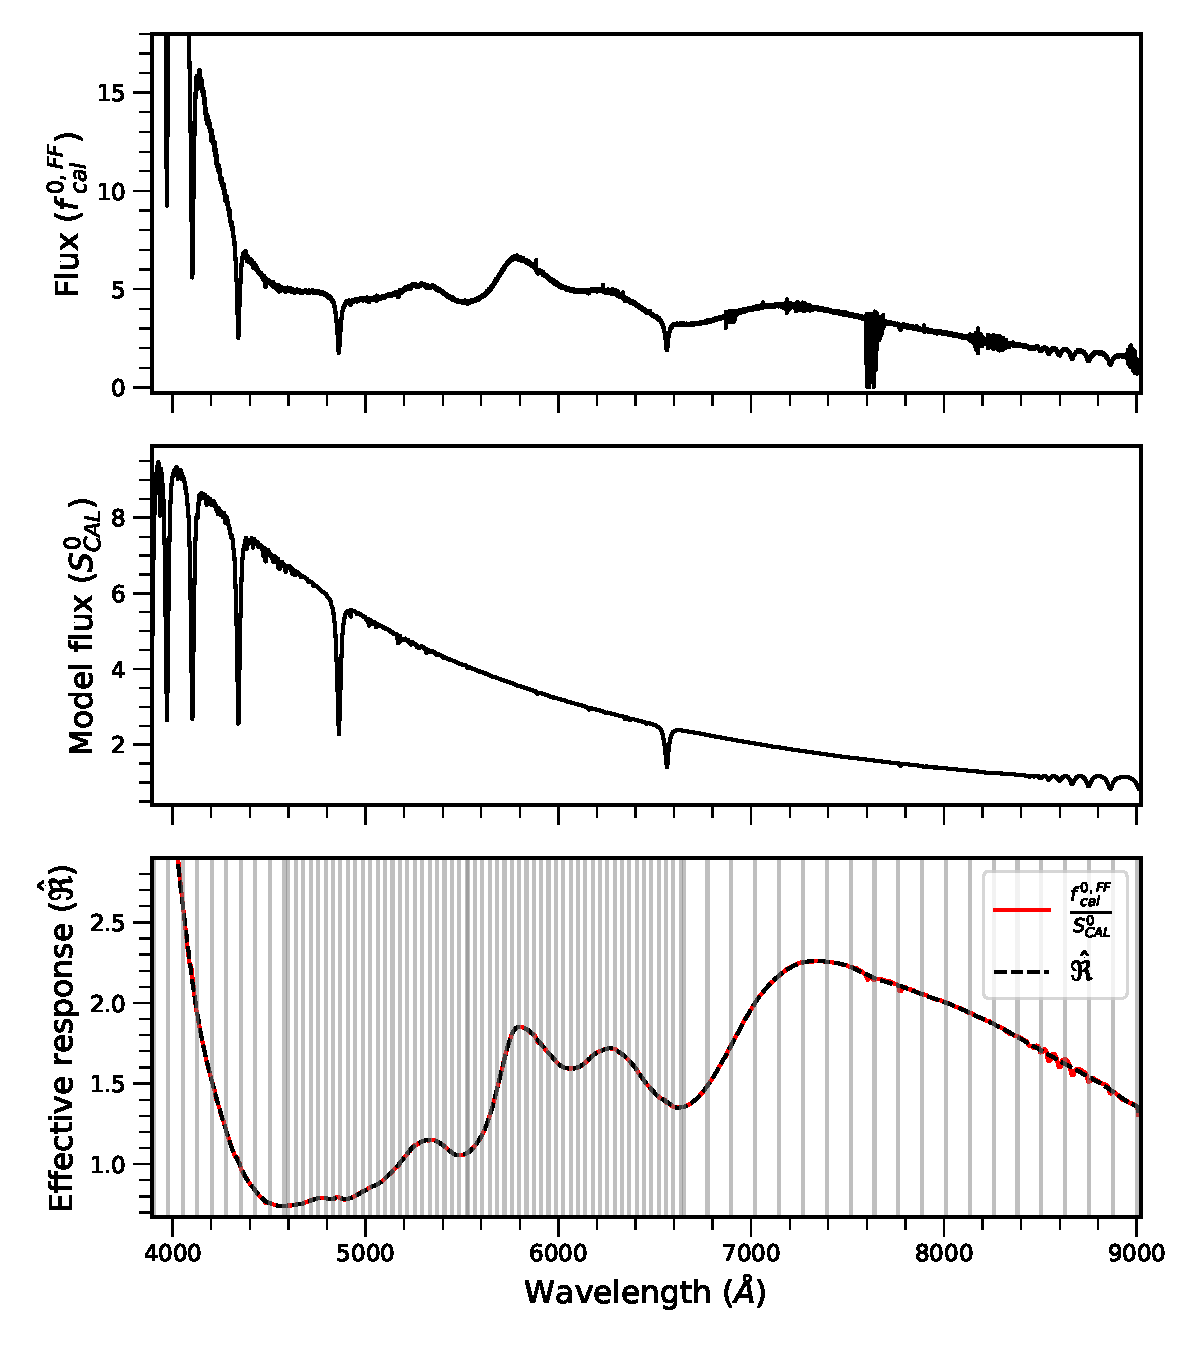
\includegraphics[width=\hsize]{chapters/data_reduction/image/ResponseDerivation.pdf}
     \caption{The derivation of the effective response for a night (Eq. \ref{eqn:hatre}). The spectrophotometric calibrator star used in this example is HD 42818. \textbf{Top:} the spectrum corrected for flat-field and atmospheric effects ($ f_{cal}^{0,FF}$). \textbf{Middle:} Model SED used to derive the response ($S^0_{CAL}$). Bottom: The derived effective response ($\hat{\Re}$) in red which is fit with a spline in black. The knot points used to fit the spline are shown with vertical grey lines. }
     \label{fig:respDerivation}
\end{figure}

\subsection{Response correction}
\label{sec:responsecorr}

At this stage, the spectra can be expressed as:
    \begin{align}
    \label{eq:divff0obj}
    f_{obj}^{0,FF} &= \frac{S^0_{OBJ} .\, \Re}{ff}\\
    \label{eq:divff0cal}
    f_{cal}^{0,FF} &= \frac{S^0_{CAL} .\, \Re}{ff}
    \end{align}
where "$FF$" and "$0$" indicate that the flat-field and atmospheric corrections have been applied and $ff \triangleq FF_{SED} .\, \Re$. 

If we define an effective instrumental response $\hat{\Re}$ combining the system response with the effect of the flat-field
\begin{equation}
    \label{eqn:hatre}
    \hat{\Re} \triangleq \frac{\Re}{ff} = \frac{f^{0,FF}_{cal}}{S^0_{CAL}}
\end{equation}
we can express the final spectrum, corrected from the instrumental response, the effects induced by the flat-field correction and the effects from the atmosphere as:
\begin{equation}
\label{eqn:Sfinal}
%S^0_{OBJ} = f^{0,FF}_{obj} .\, \frac{ff}{\Re} = f^{0,FF}_{obj} .\, \frac{S^0_{CAL}}{f^{0,FF}_{cal}}
S^0_{OBJ} = \frac{f^{0,FF}_{obj}}{\hat{\Re}}
\end{equation}


One spectrophotometric standard was observed every night when possible as part of the normal calibration set of HERMES, aiming at a daily determination of $\hat{\Re}$. These targets were carefully selected for this purpose: they are well documented in the literature, and have reliable models established by a series of independent publications. All of these targets were modelled with the LTE model-atmosphere code \textsc{gssp} \citep{tkachenko_grid_2015}. \textsc{gssp} generates synthetic spectra using the \textsc{SynthV} radiative transfer code \citep{tsymbal_starsp_1996} combined with a grid of atmospheric models from the \textsc{LLmodels} code \citep{shulyak_line-by-line_2004}. These synthetic spectra are then fitted to the highest-SNR observed spectrum for each star in the HERMES archive. The atmospheric parameters $T_{\text{eff}}$, log $g$, projected rotational velocity ($\varv$~sin~$i$), microturbulent velocity ($\varv_{\text{mic}}$) and the metallicity ($\mathrm{[M/H]}$) and their corresponding uncertainties were then determined from the distribution of $\chi^{2}$ values of the fit of each synthetic spectrum to the observed spectrum. We then used the closest parameters in the \textsc{LLmodels} grid to our best-fitting values as the input to generate the spectral energy distribution (SED) models of our calibrators. 

The result of the division of the calibrator spectrum by the model in Eq.~\ref{eqn:hatre} is first smoothed with a median filter and then fit with a spline in order to produce a smooth, yet accurate representation of the effective response ($\hat{\Re}$) before injecting it in Eq.~\ref{eqn:Sfinal}, hence avoiding the introduction of noise resulting from the observation of the calibration star or local residuals from its model in the corrected spectra. The density of knot points used to fit the spline are chosen locally depending on the complexity of the response (bottom panel of Fig. \ref{fig:respDerivation}). All spectra obtained over the corresponding night are then divided by this response, resulting in a reliable representation of the continuum shape. 
In a few cases where a spectrophotometric standard was not observed, the effective response derived for the nearest night in time was then used instead. It is important to note that the shape of the flat-field affects the effective response. This change in the $FF_{SED}$ depends on the temperature of the lamps, which is not monitored. Hence, we have no control over the applicability of a given response (derived from another night) to a given night. As a result, a few of the response corrections are inaccurate on such nights, leaving characteristic low-frequency signatures in the spectra. 

The output of the response correction are HERMES spectra whose shapes represent the star's SED. Although the spectra are not flux-calibrated, we are able to use continuum models to normalise these spectra. In the Chapters 3, 4 and 5, we will use this technique to reduce all of our observations of WR stars. Furthermore, the calibration techniques presented in this chapter have been deployed and applied to the entire HERMES archive (3258 spectra, 478 nights) in the context of an upcoming data release of the Mercator Library of High-Resolution Stellar Spectroscopy (Royer, Dsilva et. al in prep). 

%\textbf{(2539/3259 for when we have meteo data $\geq$2010-09-27, double checked with STDNIGHT)}.
%Correcting a spectrum with a response estimated from the wrong family produces characteristic features in the corrected spectra, allowing to design a new selection criterion for the effective response, now taken from 'the nearest night from the same family'.



% \begin{comment}
% \begin{figure}[ht]
% \centering
% \includegraphics[width=\hsize]{Molecfit_correction.pdf}
%      \caption{A spectrum of HD\,3379 (B2.5IV) focusing on the telluric correction with {\tt molecfit}.}
%      \label{fig_mfitcorr}
% \end{figure}
% \end{comment}

% \begin{figure}
% \centering
% \includegraphics[width=\hsize]{fig_molec_307775.png}
%      \caption{The effect of the telluric correction on a spectrum from HD\,19356 (B8V). In red, before the correction. In black, after {\tt molecfit}. The insert shows the region around $H\alpha$. Whereas weak lines are usually very well corrected, large correction residuals do appear at the level of saturated telluric lines.}
%      \label{fig_mfitcorr}
% \end{figure}

